% !TeX root = ../tesis.tex

\chapter{Teoría}
\label{chapter:Teoria}

\vspace{2cm}

En este capítulo se estudia la interacción de la luz con la materia, caracterizada por una función dieléctrica dependiente de la frecuencia, que se modifica según el tamaño del objeto. En la primera sección se presentan la  solución de ondas planas a las ecuaciones de Maxwell y las condiciones que se imponen a los campos electromagnéticos (EMs) al propagarse a través de un medio homogéneo, lineal e isótropo, y al cruzar una interfaz arbitraria a otro medio con las mismas características, así como el caso particular de la reflexión y transmisión de una onda plana al cruzar una interfaz plana, que deviene en las fórmulas de Fresnel. En la segunda sección se presenta la solución de Mie, que consiste en la solución al problema de absorción y esparcimiento de luz debido a una partícula esférica de tamaño y material arbitrario al ser iluminada por una onda plana monocromática, dando como resultado los campos EMs esparcidos por la partícula. En la tercera sección se presenta el modelo de Drude-Sommerfeld para la función dieléctrica como respuesta EM de materiales plasmónicos, así como un método para ajustar las mediciones experimentales de la función dieléctrica y poder hacer la corrección de tamaño para partículas esféricas \emph{pequeñas}; asimismo se definen los plasmones ---acoplamiento de la luz con los electrones libres de un material--- al considerar materiales cuya respuesta EM es descrita por el modelo de Drude-Sommerfeld, así como el caso de materiales más realistas (oro y plata). Finalmente, en la cuarta sección, se presenta la respuesta EM de una monocapa de partículas esféricas idénticas, descrita por el modelo de esparcimiento coherente (Coherent Scattering Model, CSM) en donde se calculan los coeficientes de amplitud de reflexión y transmisión para un sistema monocapa de NPs esféricas idénticas, inmersa en un medio dieléctrico (denominado matriz) y soportada por un sustrato dieléctrico.

\section{Ecuaciones de Maxwell y fórmulas de Fresnel}
\label{section:NocionesBasicas}

Las ecuaciones de Maxwell  describren, junto con la fuerza de Lorentz, toda la electrodinámica y en su forma diferencial están dadas por las siguientes expresiones \cite{griffiths2013electrodynamics}:  \index{Maxwell!ecuaciones de} \vspace*{-.75em}
%
	\begin{subequations} \label{eqs:Maxwell}
	\begin{tcolorbox}[title = Ecuaciones de Maxwell en el sistema internacional de unidades,
	ams align, breakable]
	\nabla \cdot\vb{E} &= \frac{\rho_{tot}}{\varepsilon_0}, &\mbox{(Ley de Gauss eléctrica)}  
	\label{seq:GE} \\
	\nabla \cdot\vb{B} &= 0,						&\mbox{(Ley de Gauss magnética)}   
	\label{seq:GM} \\
	\nabla \times\vb{E} &= -\pdv{\vb{B}}{t}, 	&\mbox{(Ley de Faraday-Lenz)}		
	\label{seq:FL}\\
	\nabla \times\vb{B} &= \mu_0 \vb{J}_{tot} +\varepsilon_0\mu_0 \pdv{\vb{E}}{t}, &
	\mbox{(Ley de Ampère-Maxwell)} \label{seq:AM}
	\end{tcolorbox}\end{subequations}\vspace*{-.75em}\noindent
%
%	\begin{subequations} \label{eqs:Maxwell}
%	\begin{tcolorbox}[title = Ecuaciones de Maxwell en el sistema internacional de unidades,
%	ams align, breakable]
%	\nabla \cdot\vb{E} &= \frac{\rho_{tot}}{\varepsilon_0}, &\mbox{(Ley de Gauss eléctrica)}  \label{seq:GE} \\
%	\nabla \cdot\vb{B} &= 0,						&\mbox{(Ley de Gauss magnética)}   \label{seq:GM} 
%\end{tcolorbox}	\begin{tcolorbox}[title = Ecuaciones de Maxwell en el sistema internacional de unidades,ams align, breakable]
%	\nabla \times\vb{E} &= -\pdv{\vb{B}}{t}, 	&\mbox{(Ley de Faraday-Lenz)}		\label{seq:FL}\\
%	\nabla \times\vb{B} &= \mu_0 \vb{J}_{tot} +\varepsilon_0\mu_0 \pdv{\vb{E}}{t}, & \mbox{(Ley de Ampère-Maxwell)} \label{seq:AM}
%	\end{tcolorbox}\end{subequations}\vspace*{-.75em}\noindent
%
donde $\vb{E}$ es el campo eléctrico y $\vb{B}$, el campo magnético; $\rho_{tot}$ es la densidad volumétrica de carga total  y $\vb{J}_{tot}$, la densidad volumétrica de corriente total; $\varepsilon_0$ es la permitividad eléctrica del vacío y $\mu_0$, la permeabilidad magnética del vacío.

Al desacoplar las ecuaciones de Maxwell, los campos EMs obedecen la ecuación de onda \cite{hecht1998optics}, \index{Ecuación!de onda} que al emplear la transformada Fourier\footnote{\setstretch{1.0} $\mathcal{F}[f(\vb{r},\omega)] = \int_{-\infty}^\infty f(\vb{r},t) e^{i(\vb{k}\cdot\vb{r} -\omega t)} dt$, con $\vb{k}$ una función de $\omega$. La transformada de Fourier inversa es entonces $\mathcal{F}^{-1}[f(\vb{r},t)] =\frac{1}{2\pi} \int_{-\infty}^\infty f(\vb{r},\omega) e^{i(\vb{k}\cdot\vb{r} -\omega t)} d\omega$.\index{Fourier!transformada de}} y considerar una región del espacio sin fuentes ($\rho_{tot}=0$ y $\vb{J}_{tot}=\vb{0}$), se obtiene la ecuación de Helmholtz \index{Ecuación!de Helmholtz} para $\vb{E}$ y $\vb{B}$ \cite{griffiths2013electrodynamics}

	\begin{subequations}\eqhalf{\nabla^2\vb{E} + k^2 \vb{E}=\vb{0},}
	\eqhalf{\nabla^2\vb{B} + k^2 \vb{B}=\vb{0}.}\label{eq:Helmholtz}\end{subequations}\vspace*{-1em}

\noindent Una de las soluciones a la ecuación de Helmholtz para los campos EMs son las ondas planas, es decir, que los campos EMs son de la forma \cite{jackson1999electrodynamics} \index{Maxwell!ecuaciones de!solución de ondas 
planas a las}\index{Onda!plana}\index{Onda!plana!en la base cartesiana canónica}

	\begin{subequations}\eqhalf{\vb{E}(\vb{r},t) =\vb{E_0}e^{i(\vb{k}\cdot\vb{r} -\omega t)},}
	\eqhalf{\vb{B}(\vb{r}, t) =\vb{B_0}e^{i(\vb{k}\cdot\vb{r} -\omega t),}}	
	\label{eqs:ondasPlanas}\end{subequations}\vspace*{-1em}
		
\noindent en donde  $\vb{E_0}$ y $\vb{B_0}$ representan las amplitudes de los campos EMs, $\vb{k}$ es el vector de onda y $\omega$ es la frecuencia angular; la tríada de vectores \{$\vb{k},\, \vb{E},\, \vb{B}$\} constituye una base ortogonal derecha en el vacío \cite{griffiths2013electrodynamics}. Para un medio material caracterizado por una función dieléctrica $\varepsilon(\omega)$ y una permeabilidad magnética $\mu$, se define el índice de refracción del medio $n(\omega)$ como \index{Índice de refracción}\index{Índice de refracción|seealso{Función dieléctrica}}\index{Función dieléctrica}\vspace*{-.75em}
%
	\begin{tcolorbox}[title = Índice de refracción, ams align]
	n(\omega) = \sqrt{\frac{\mu\varepsilon(\omega)}{\varepsilon_0 \mu_0}}.
		\label{eq:indice} 
	\end{tcolorbox}\vspace*{-.75em}\noindent
%
Tanto $n(\omega)$, como $\varepsilon(\omega)$ y $\mu$ se determinan de forma experimental y son, en general, cantidades complejas. Para que las ondas planas sean solución de las ecuaciones de Maxwell, es necesario que se cumpla la relación de dispersión, que relaciona a  la magnitud del vector de onda $k$ con la frecuencia angular $\omega$ de la siguiente manera \vspace*{-.75em}\index{Relación de dispersión}\index{Relación de dispersión!de una onda plana}
%
	\begin{tcolorbox}[title = Relación de dispersión, ams align]
	k(\omega) = \frac{\omega}{c}n(\omega),
	\label{eq:dispersion}
	\end{tcolorbox}\vspace*{-.75em}\noindent
%
en donde  $c=\sqrt{1/\varepsilon_0\mu_0}$ es la velocidad de la luz.

A partir de las ecuaciones de Maxwell se construye el teorema de conservación de la energía \cite{griffiths2013electrodynamics}, escrito en términos del vector de Poynting $\vb{S}$\index{Poynting!vector de}, que representa el flujo de energía EM por unidad de tiempo y unidad de área. Al considerar campos EMs de la forma de ondas planas [Ec. \eqref{eqs:ondasPlanas}], el vector de Poynting está dado por \cite{hecht1998optics}\vspace*{-.75em}
%
	\begin{tcolorbox}[title = Vector de Poynting, ams align]
	\vb{S} = \vb{E}\times\vb{H}^*,  \label{eq:Poynting}
	\end{tcolorbox} \vspace*{-.75em}\noindent
%
en donde $\vb{H}=\vb{B}/\mu$ es el campo H y $*$ corresponde a la operación complejo conjugado.

Las ecuaciones de Maxwell imponen condiciones a la frontera sobre los campos EMs cuando estos cruzan la frontera entre dos medios distintos, denominada interfaz. En la Fig. \ref{fig:GaussAmpere} se muestra la interfaz entre dos medios arbitrarios caracterizados por la función dieléctrica $\varepsilon_i$ y la permeabilidad magnética $\mu_i$, con $i = 1,\,2$ dependiendo del medio. Para deducir las condiciones a la frontera de los campos EMs sobre la interfaz, con vector normal $\vu{u}$, se evalúan los campos EMs en un cilindro con caras de área $A$ y altura $\delta$ [ver Fig. \ref{sfig:GaussPillbox}], así como  en un circuito de largo $l$ y altura $\delta$ [ver Fig. \ref{sfig:AmperianLoop}]. Al considerar el límite $\delta \to 0$, evaluando los campos EMs sobre la interfaz, la ausencia de fuentes externas ($\sigma_{ext} = 0$ y $\vb{K}_{ext} = \vb{0}$) y que los medios que conforman a la interfaz son lineales, homogéneos e isótropos, los campos EMs obedecen las  siguientes condiciones \cite{griffiths2013electrodynamics}:\vspace*{-.75em}\index{Electromagnéticos!campos!condiciones a la frontera de los}
%
	\begin{subequations}
	\begin{tcolorbox}[title = Condiciones de frontera de los campos EMs sin fuentes externas]
	\eqhalf{\varepsilon_1 E^\perp_1 - \varepsilon_2 E^\perp_2 = 0, \label{seq:Eperp}}
	\eqhalf{\vb{E}_1^\parallel -\vb{E}_2^\parallel = \vb{0},\label{seq:Epara}}\vspace*{.5em}
	\eqhalf{B_1^{\perp} - B_2^{\perp} = 0, \label{seq:Bperp} }
	\eqhalf{\frac{\vb{B}^\parallel_1}{\mu_1} - \frac{\vb{B}^\parallel_2}{\mu_2} =\vb{0},\label{seq:Bpara}} 
	\end{tcolorbox} \label{eqs:CFrontera}	\end{subequations}\vspace*{-.75em}\noindent
	%
donde $\perp$ corresponde a la componente perpendicular a la interfaz y $\parallel$, a la paralela.
%
	\begin{figure}[h!]\centering
	\begin{subfigure}{.05\textwidth}\vspace{-3cm}\caption{}\label{sfig:GaussPillbox}	\end{subfigure}
	\begin{subfigure}{.43\textwidth} \hspace*{-1cm}
\begin{tikzpicture}[scale=1]
%\draw (3.46,1.9) circle(2pt);ESTA ES LAREFERENCIA PARA ANTES DE MOVER LAS COSAS

%%%%%%%%%%%%%%%%%%%%%%%%%%%%%%%%%%%%%%%%%%%%%%%% 	SUPERFICIE
\shadedraw[	top color =lblue,				%%%%	Color de arriba
			bottom color =lblue,				%%%%	Color de abajo
			middle color = bone, 			%%	Color de en medio
			shading angle = -22]			%%%%	Ángulo de gradiente
			
(-1,1) ..controls (2, 0) and (3,3.5) .. (4.5,3.5) %	Aquí se dan las lineas
-- (7,3.2) .. controls (5,3) and (4,-.5) .. (2.5,.5)%	A .. ctrls P and Q.. B 
--(-1,1);								%%%%%%%%%	P y Q jalan la linea de A a B
\node[color = black] at (3,.6) { $\sigma_{tot}$};
\node  at (0,1.2) {\small Medio 1};
\node at (0,.3) {\small Medio 2};

%%%%%%%%%%%%%%%%%%%%%%%%%%%%%%%%%%%%%%%%%%%%%%%%%%%%%%%%%	PILL-BOX
\fill[dgreen, opacity = .3]						%%%%%%%%	Cara del cilindro
 (3.46-.7,2.05) arc(180: 0: .7 and .2)			%%%%%%%% 	se pone el principio pero es
-- (3.46+.7,1.75) arc(0: -180: .7 and .2)		%%%%%%%		lo ultimo que puedo escribir
-- (3.46-.7,2.05);

\draw[black](3.46,2.05) circle (.7 and .2)		%%%%%%		Centro y radios de curvatura
(4.1,2.15)node[above]{ $A$};	%%%%		Etiqueta del área
\fill[dgreen, opacity = .1] (3.46,2.05) circle (.7 and .2); 

\draw[black](3.46,1.9)  circle (.7 and .2);
\fill[dgreen,opacity = .1](3.46,1.9)  circle (.7 and .2);

\draw[densely dotted, black](3.46,1.75)  circle (.7 and .2);
\fill[dgreen,opacity = .1](3.46,1.75)  circle (.7 and .2);

\draw[black, line width = .2mm]						%%%%%%	Lineas que faltó llenar
(3.46-.7,2.05) -- (3.46-.7,1.9)		(3.46+.7,2.05) -- (3.46+.7,1.9);
\draw[densely dotted, black, line width = .2mm]
(3.46-.7,1.9) -- (3.46-.7,1.75)		(3.46+.7,1.9) -- (3.46+.7,1.75);
 
  
%%%%%%%%%%%%%%%%%%%%%%%%%%%%%%%%%%%%%%%%%%%%%%%%%%%%%%%%%%%%	VECTOR NORMAL (Perp)
%\draw[ -latex ,line width=.2mm, black]	
% (3.46,2.05)--(3.46,2.6+.1);	%%%%	Se toma un punto medio y se desplaza para dar profundidad
%\node[color = black, right] at (3.46-.1,2.6+.2) { $\vb{a}_\perp$};%	Se etiqueta la flecha

\draw[ -latex ,line width=.2mm, black]	
 (3.46,2.05)--(3.46,2.6+.1);	%%%%	Se toma un punto medio y se desplaza para dar profundidad
\node[color = black, right] at (3.46-.1,2.6+.2) { $\vu{u}$};%	Se etiqueta la flecha

%%%%%%%%%%%%%%%%%%%%%%%%%%%%%%%%%%%%%%%%%%%%%%%%%%%%%%%%%%%%	VECTOR NORMAL (Paralelo)
%\draw[-latex ,line width=.2mm, black]	
% (3.46-.7+.3, 1.9-.15)-- (3.46-.7-.1,1.95-.4);	
%\node[color = black, left] at (3.46-.1,1.95-.6) { $\vb{a}_\parallel$};%	Se etiqueta la flecha

%%%%%%%%%%%%%%%%%%%%%%%%%%%%%%%%%%%%%%%%%%%%%%%%%%%%%%%%%	LINEA DE ALTURA
\draw[|-, line width=.2mm,black]
(3.46+.7+.15,2.05) -- (3.46+.7+.15, 1.9);
\draw[-|, densely dotted, line width=.2mm,black]
(3.46+.7+.15,1.9) -- (3.46+.7+.15,1.7);
\node[color = black, right] at (3.46+.7+.15,1.9) { $\delta$};
\end{tikzpicture}	
	\end{subfigure}
	\begin{subfigure}{.05\textwidth}\vspace{-3cm}\caption{}\label{sfig:AmperianLoop}\end{subfigure}
	\begin{subfigure}{.43\textwidth}  \hspace*{-1cm}
\begin{tikzpicture}[scale=1]
%--------------------------------------------------- 	SUPERFICIE

\shadedraw[	top color =lblue,				%		Color de arriba
			bottom color =lblue,				%		Color de abajo
			middle color = bone, 			%		Color de en medio
			shading angle = -18]			%		Ángulo de gradiente
			
	(-1,1) ..controls (2, 0) and (3,3.5) .. (4.5,3.5) %	Aquí se dan las lineas
	-- (7,3.2) .. controls (5,3) and (4,-.5) .. (2.5,.5)%	A .. ctrls P and Q.. B 
	--(-1,1);								%%%%%%%%%	P y Q jalan la linea de A a B

\node[color = black] at (3,.7) { $\vb{K}_{tot}$};
\node  at (0,1.2) {\small Medio 1};
\node at (0,.3) {\small Medio 2};
\draw[- latex, thick, shift={(-.2,.15)}]  (2.4,.78)  -- (1.4,.9) ;  
\draw[- latex, thick, shift={(-.2,.15)}]  (2.7,.88)  -- (1.7,1) ; 
\draw[- latex, thick, shift={(-.2,.15)}]  (3,.98)  -- (2,1.1) ; 

%---------------------------------------------------	CIRCUITO
\draw[densely dotted, line width=.2mm,black, reverse directed] 
(3.0,1.4)-- (3.92,2.4)
		-- (3.92,2.1)
		-- (3.0,1.1)
		-- (3.0,1.4);
\draw[line width=.2mm, black, directed] 
(3.0,1.4)--(3.92,2.4)		 
 		-- (3.92,2.7)		
 		-- (3.0,1.7) 
 		-- (3.0,1.4);
 							%%%%%%%%%	Estos ultimos son para colorear el circuitp
\fill[dgreen,opacity = .3] (3.0,1.4)--(3.92,2.4)-- (3.92,2.7)-- (3.0,1.7)-- (3.0,1.4);
\fill[dgreen,opacity = .2](3.0,1.1)--(3.92,2.1)-- (3.92,2.4)-- (3.0,1.4)-- (3.0,1.1);
 
%---------------------------------------------------	VECTOR NORMAL
\draw[ - latex ,line width=.2mm, black]	
 (3.46,1.9)--(3.46,2.6);	%%%%	Se toma un punto medio y se desplaza para dar profundidad
\path (3.5,2.5) node[color = black, above]{ $\vu{u}$};%	Se etiqueta la flecha

%---------------------------------------------------      LINEA DE LONGITUD
\draw[|-|,line width=.2mm,black] (3.08+.1,1.1-.1)--(4+.1,2.1-.1);%		Se escogieron puntos arbitrarios
\path (3.34+.4 ,1.8-.4) node[color = black]{ $l$}  ;%	Se toma el punto medio y se traslada

%---------------------------------------------------	LINEA DE ALTURA
\draw[|-, densely dotted, line width=.2mm,black] (3.92+.2,2.1+.1)--(3.92+.2,2.4+.1);
\draw[-|, line width=.2mm,black] (3.92+.2,2.4+.1)--(3.92+.2,2.7+.1);
\path (3.92+.2,2.4+.1) node[color = black, right]{ $ \delta$};
\end{tikzpicture}
	\end{subfigure} \vspace*{-.7cm}
	\caption{Esquema de una interfaz entre dos medios distintos y arbitrarios con {\bf a)} una densidad de carga superficial $\sigma_{tot}$ y {\bf b)} una densidad de corriente superficial $\vb{K}_{tot}$. Los campos EMs son evaluados en \textbf{a)} en el cilindro de área $A$ y altura $\delta \to 0$ y en \textbf{b)} en el circuito de largo $l$ y altura $\delta\to 0$. En ambas figuras el vector normal a la superficie es $\vu{u}.$}	\label{fig:GaussAmpere}	
	\end{figure}	
				
Cuando una onda plana [Ec. \eqref{eqs:ondasPlanas}] incide sobre la interfaz entre dos medios lineales, homogéneos e isótropos, ésta se descompone en una onda plana reflejada y una transmitida. Al describir el medio de incidencia y de transmisión por su índice de refracción $n_i$ y $n_t$, respectivamente, e imponer las condiciones a la frontera del los campos EMs [Ecs. \eqref{eqs:CFrontera}], válidas para todo tiempo y todo punto en la interfaz, las fases de las tres ondas son iguales, por lo que se cumple: \vspace*{-.75em} \index{Ley!de la reflexión}\index{Ley!de Snell}
%
	\begin{tcolorbox}[title = Ley de reflexión y ley de Snell ]
	\eqhalf{\theta_i = \theta_r,  \label{eq:LeyReflexion}}
	\eqhalf{ n_i \sin\theta_i = n_t \sin\theta_t,\label{eq:LeySnell}}
	\end{tcolorbox}	 \vspace*{-.75em}\noindent
%
en donde $\theta_i$ es el ángulo de incidencia; $\theta_r$, el de reflexión y $\theta_t$, el de transmisión; los tres medidos respecto la dirección normal a la interfaz. La Ec. \eqref{eq:LeyReflexion} es la llamada ley de reflexión mientras que la Ec. \eqref{eq:LeySnell} es conocida como la ley de Snell\footnote{La ley fue nombrada así debido al físico holandés Willebroerd Snellius, aunque investigaciones más recientes indican que el registro más antiguo de esta ley (correctamente formulada) fue en el año 984 en el libro \emph{On the Burning Instruments} del matemático persa Ibn Sahl \cite{kwan2002really}.}, y determinan la dirección de propagación de las ondas planas reflejada y el transmitida.

Los coeficientes de amplitud de reflexión $r$ y de transmisión $t$ se definen como el cociente de las amplitudes del campo eléctrico reflejado $E^r$, y transmitido $E^t$, respectivamente, entre el campo eléctrico incidente $E^i$ \index{Fresnel!ecuaciones de}. El valor de los coeficientes de amplitud $r$ y $t$ depende de la polarización del campo eléctrico incidente, es decir, de la dirección en la que $\vb{E}^i$ oscila respecto al plano definido por el vector normal a la interfaz y la dirección de propagación de la onda plana incidente, denominado plano de incidencia\index{Plano!de incidencia}. En la Fig. \ref{fig:Polarizaciones} se muestra una onda plana que se propaga en el medio de incidencia (con índice de refracción $n_i$) en la dirección $\vb{k}^i$, e incide sobre la interfaz a un ángulo $\theta_i$ respecto al vector normal a la interfaz. La onda plana se refleja con un ángulo $\theta_r = \theta_i$ y se propaga en una dirección $\vb{k}^r$, y también se refracta en un ángulo $\theta_t$, dado por la Ec. \eqref{eq:LeySnell}, y se propaga en una dirección $\vb{k}^t$. En la Fig. \ref{sfig:Pols} el campo eléctrico oscila en dirección perpendicular al plano de incidencia, por lo que se le denomina polarización \emph{s} (del alemán \emph{senkrecht}), mientras que en la Fig. \ref{sfig:Polp} el campo eléctrico oscila paralelo al plano de incidencia, por lo que se le denomina polarización \emph{p} (del alemán \emph{parallel}).\index{Fresnel!coeficientes de amplitud de ($r,t$)}
 \index{Polarización!de una onda plana}\index{Polarización!respecto al plano de incidencia!paralela (\emph{p})}\index{Polarización!respecto al plano de incidencia!perpendicular (\emph{s})}
%
	\begin{figure}[h!]\centering
	\begin{subfigure}{.05\textwidth}\vspace{-4.5cm}\caption{}\label{sfig:Pols}\end{subfigure}
	\begin{subfigure}{.43\textwidth} \hspace*{-1cm}
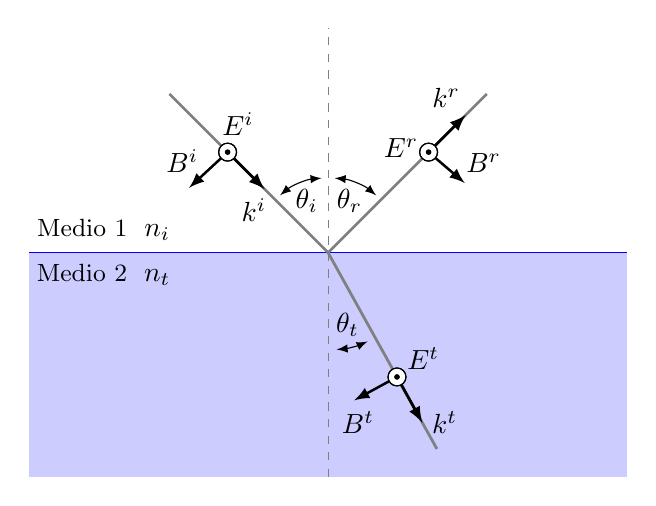
\begin{tikzpicture}[scale=.95]

%-------------------------------------------- Incidence media
\fill[blue!20] (-4,-3) rectangle (4,0);
% Interface
\draw[blue,line width=.5pt](-4,0)--(4,0); %%..5pt, interface]
% Vertical dashed line
\draw[dashed,gray,](0,-3)--(0,3);
% Media names
\node at (-3,.3) {{\small Medio 1} $\; n_i$}; 
\node at (-3,-.3) {{\small Medio 2} $\; n_t$};

%--------------------------------------------  Incident Wave
\draw[gray, line width=1pt](0:0cm)--(135:3cm);  % Light trajectory
\path (0,0)++(112.5:.75cm)node{$\theta_i$};       % Angle
\draw[latex-latex](95:1.cm)arc(95:130:1.cm);
 
    \draw[-latex,line width=1pt](135:1.9cm)--(135:1.2cm);    %Wave vector
    \path (0,0)++(141:0.9cm)node[left]{$\vb{k}^i$};     %Wave vector label
    
    \draw[-latex,line width=.9pt](135:1.9cm)--(155:2.05cm);  %B vector
    \path (0,0)++(148:2.3cm)node{$\vb{B}^i$}; 
    
    \path (0,0)++(125:2.1cm)node{$\vb{E}^i$};       % E vector
    
    \draw [fill= white](135:1.9cm)circle (0.12cm); % Vector perp. to surface
    \draw [black](135:1.9cm)circle (0.12cm);
    \filldraw[fill=black](135:1.9cm) circle(0.03cm); %%
    
%--------------------------------------------  Reflected Wave
\draw[gray,line width=1pt](0:0cm)--(45:3cm);  % Light trajectory
\path (0,0)++(67.5:.75cm)node{$\theta_r$};       % Angle
\draw[latex-latex](85:1.cm)arc(85:50:1.cm);
 
    \draw[-latex,line width=1pt](45:1.9cm)--(45:2.6cm);    %Wave vector
    \path (0,0)++(47.5:2.8cm)node[left]{$\vb{k}^r$};     %Wave vector label
    
    \draw[-latex,line width=.9pt](45:1.9cm)--(27:2.05cm);  %B vector
    \path (0,0)++(30:2.4cm)node{$\vb{B}^r$}; 
    
    \path (0,0)++(55:1.7cm)node{$\vb{E}^r$};       % E vector
    
    \draw [fill= white](45:1.9cm)circle (0.12cm); % Vector perp. to surface
    \draw [black](45:1.9cm)circle (0.12cm);
    \filldraw[fill=black](45:1.9cm) circle(0.03cm); %%

%--------------------------------------------  Transmitted Wave
\draw[gray,line width=1pt](0:0cm)--(-61:3cm);  % Light trajectory
\path (0,0)++(-75:1cm)node{$\theta_t$};       % Angle
\draw[latex-latex](-85:1.3cm)arc(-85:-66:1.3cm);
 
    \draw[-latex,line width=1pt](-61:1.9cm)--(-61:2.6cm);    %Wave vector
    \path (0,0)++(-61:2.6cm)node[right]{$\vb{k}^t$};     %Wave vector label

    \draw[-latex,line width=.9pt](-61:1.9cm)--(-80:2.005cm);  %B vector
    \path (0,0)++(-80:2.3cm)node{$\vb{B}^t$}; 
    
    \path (0,0)++(-48:1.9cm)node{$\vb{E}^t$};       % E vector
    
    \draw [fill= white](-61:1.9cm)circle (0.12cm); % Vector perp. to surface
    \draw [black](-61:1.9cm)circle (0.12cm);
    \filldraw[fill=black](-61:1.9cm) circle(0.03cm); %%     
 
\end{tikzpicture}
	\end{subfigure}
	\begin{subfigure}{.05\textwidth}\vspace{-4.5cm}\caption{}\label{sfig:Polp}	\end{subfigure}
	\begin{subfigure}{.43\textwidth}  \hspace*{-1cm}
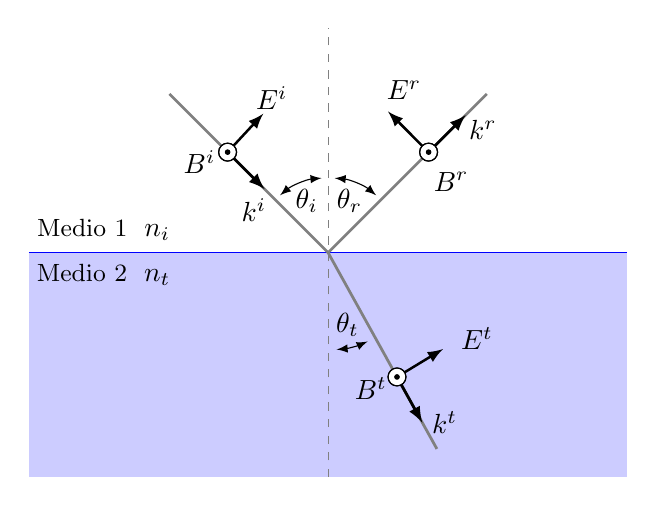
\begin{tikzpicture}[scale=.95]
%-------------------------------------------- Incidence media
\fill[blue!20] (-4,-3) rectangle (4,0);
% Interface
\draw[blue,line width=.5pt](-4,0)--(4,0); %%..5pt, interface]
% Vertical dashed line
\draw[dashed,gray,](0,-3)--(0,3);
% Media names
\node at (-3,.3) {{\small Medio 1} $\; n_i$}; 
\node at (-3,-.3) {{\small Medio 2} $\; n_t$};

%--------------------------------------------  Incident Wave
\draw[gray, line width=1pt](0:0cm)--(135:3cm);  % Light trajectory
\path (0,0)++(112.5:.75cm)node{$\theta_i$};       % Angle
\draw[latex-latex](95:1.cm)arc(95:130:1.cm);
 
    \draw[-latex,line width=1pt](135:1.9cm)--(135:1.2cm);    %Wave vector
    \path (0,0)++(141:0.9cm)node[left]{$\vb{k}^i$};     %Wave vector label
    
    \draw[-latex,line width=.9pt](135:1.9cm)--(115:2.05cm);  %E vector
    \path (0,0)++(110:2.2cm)node{$\vb{E}^i$}; 
%    \draw[-latex,line width=.9pt, red]((135:1.9cm)--(117:1.55cm); 

    
    \path (0,0)++(145:2.1cm)node{$\vb{B}^i$};       % B vector
    
    \draw [fill= white](135:1.9cm)circle (0.12cm);
    \draw [black](135:1.9cm)circle (0.12cm);
    \filldraw[fill=black](135:1.9cm) circle(0.03cm); %%    
    
    
%    \draw[line width=.6pt] (135:1.9cm)   % Esto esra paea hacer el vector salir de la hoja
%                         +(-135:.12cm) -- +(45:.12cm)
%                         +(-45:.12cm) -- +(135:.12cm);    
   
    
%--------------------------------------------  Reflected Wave
\draw[gray,line width=1pt](0:0cm)--(45:3cm);  % Light trajectory
\path (0,0)++(67.5:.75cm)node{$\theta_r$};       % Angle
\draw[latex-latex](85:1.cm)arc(85:50:1.cm);
 
    \draw[-latex,line width=1pt](45:1.9cm)--(45:2.6cm);    %Wave vector
    \path (0,0)++(43:2.4cm)node[right]{$\vb{k}^r$};     %Wave vector label
    
    \draw[-latex,line width=.9pt](45:1.9cm)--(67:2.05cm);  %E vector
    \path (0,0)++(65:2.4cm)node{$\vb{E}^r$};
  %  \draw[-latex,line width=.9pt, red](45:1.9cm)--(59:1.55cm); 
   % \draw[dashed,red,line width=.9pt](59:1.55cm)--(67:2.05cm);
    
    \path (0,0)++(30:1.9cm)node{$\vb{B}^r$};       % B vector
    
    \draw [fill= white](45:1.9cm)circle (0.12cm);
    \draw [black](45:1.9cm)circle (0.12cm);
    \filldraw[fill=black](45:1.9cm) circle(0.03cm); %%  


%--------------------------------------------  Transmitted Wave
\draw[gray,line width=1pt](0:0cm)--(-61:3cm);  % Light trajectory
\path (0,0)++(-75:1cm)node{$\theta_t$};       % Angle
\draw[latex-latex](-85:1.3cm)arc(-85:-66:1.3cm);
 
    \draw[-latex,line width=1pt](-61:1.9cm)--(-61:2.6cm);    %Wave vector
    \path (0,0)++(-61:2.6cm)node[right]{$\vb{k}^t$};     %Wave vector label
 
    \draw[-latex,line width=.9pt](-61:1.9cm)--(-40:2.005cm);  %E vector
%      \draw[-latex,line width=.9pt, red](-61:1.9cm)--(-45:2.3cm); 
    \path (0,0)++(-30:2.3cm)node{$\vb{E}^t$}; 
    
    \path (0,0)++(-72.5:1.9cm)node{$\vb{B}^t$};       % B vector
    
    \draw [fill= white](-61:1.9cm)circle (0.12cm);
    \draw [black](-61:1.9cm)circle (0.12cm);
    \filldraw[fill=black](-61:1.9cm) circle(0.03cm); %% 
\end{tikzpicture}
	\end{subfigure} 
	\caption{ Esquema de una onda plana en polarización \textbf{a)} \emph{s} y \textbf{b)} \emph{p} que se propaga en una dirección $\vb{k}^i$ e incide con un ángulo de incidencia $\theta_i$ sobre una interfaz plana entre dos medio lineales, homogéneos e isótropos, donde el medio de incidencia tiene un índice de refracción $n_i$ y el de transmisión $n_t$. El vector de onda reflejado forma un ángulo $\theta_r=\theta_i$ con la dirección normal a la interfaz, dado por la ley de reflexión [Ec. \eqref{eq:LeyReflexion}] y el vector de onda transmitido se propaga con un ángulo $\theta_t$ dado por la ley de Snell [Ec. \eqref{eq:LeySnell}]. En el esquema se asume que la orientación de los campos EMs incidentes  ($\vb{E}^i,\,\vb{B}^i$) se preserva en los campos EMs reflejados ($\vb{E}^r,\,\vb{B}^r$) y transmitidos ($\vb{E}^t,\,\vb{B}^t$), es decir, que no hay un cambio de fase de los campos EMs al interactuar con la interfaz.}	\label{fig:Polarizaciones}	
	\end{figure}	
%

En polarización \emph{s} el campo eléctrico es perpendicular al plano de incidencia y paralelo a la interfaz por lo que, mediante la Ec. \eqref{seq:Epara}, $E^i + E^r = E^t$, en donde se asume que la orientación del campo eléctrico incidente se preserva tras la reflexión y la transmisión, como se observa en la Fig. \ref{sfig:Pols}. Al emplear la continuidad de la componente paralela a la interfaz de $\vb{B}/\mu$ [Ec. \eqref{seq:Bpara}], la relación $E = (c/n) B$, la ley de reflexión [Ec. \eqref{eq:LeyReflexion}] y de Snell [Ec. \eqref{eq:LeySnell}], así como considerar medios no magnéticos ($\mu=\mu_0$), se obtienen los coeficientes de amplitud $r$ y $t$ para  polarización \emph{s}, dados por \cite{hecht1998optics}\vspace{-.5em}
%
	\begin{tcolorbox}[title = Coeficientes de amplitud para polarización \emph{s} ]
	\vspace*{-1em}	
	\eqhalf{r_s =
		\frac{n_i\cos\theta_i-\sqrt{n_t^2-n_i^2\sin ^2\theta_i}}
 			{n_i \cos\theta_i + \sqrt{ n_t^2-n_i^2\sin ^2\theta_i}}, 
 			\label{eq:rs}}
	\eqhalf{\vspace*{-1em} t_s =
		\frac{2n_i\cos\theta_i}
 			{n_i\cos\theta_i + \sqrt{ n_t^2-n_i^2\sin ^2\theta_i}}.
 			\label{eq:ts}}
	\end{tcolorbox}	 \vspace*{-.75em}\noindent
%
Para polarización \emph{p} el campo eléctrico es paralelo al plano de incidencia, y por tanto tiene una componente paralela y una perpendicular a la interfaz, como se observa en la Fig. \ref{sfig:Polp}. Las condiciones a la frontera de los campos EM [Ec. \eqref{seq:Epara}] imponen que $E^i\cos\theta_i-E^r\cos\theta_r = E^t \cos\theta_t$. Al asumir que los campos EMs reflejado y transmitido no tienen una diferencia de fase respecto a los campos EMs incidentes, y al emplear las Ecs. \eqref{seq:Bpara},  \eqref{eq:LeyReflexion} y  \eqref{eq:LeySnell}, así como la relación $E = (c/n) B$ y considerar medios no magnéticos, se calculan los  coeficientes de amplitud $r$ y $t$ para  polarización \emph{p}, dados por \cite{hecht1998optics}\vspace*{-.75em}
%
	\begin{tcolorbox}[title = Coeficientes de amplitud para polarización \emph{p} ]
	\vspace*{-1em}
	\eqhalf{ r_p =
				\frac{n_t^2\cos\theta_i -n_i\sqrt{n_t^2-n_i^2\sin^2\theta_i}}
 				{n_t^2\cos\theta_i +n_i\sqrt{n_t^2-n_i^2\sin^2\theta_i}}, \label{eq:rp}}
	\eqhalf{\vspace*{-1em} t_p =
				\frac{ 2 n_i n_t \cos\theta_i}
 				{n_t^2\cos \theta_i+n_i\sqrt{n_t^2-n_i^2\sin^2\theta_i}}.
 				\label{eq:tp}}
	\end{tcolorbox}	\vspace*{-.75em}\noindent
%
Dado que los coeficientes  de amplitud dependen de los índices de refracción de los medios que conforman la interfaz, es posible hacer la distinción entre dos casos al analizar el término dentro de la raíz cuadrada en las Ecs. \eqref{eq:rs}--\eqref{eq:tp}: incidencia externa ($n_t>n_i$) e incidencia interna ($n_t<n_i$). En la Fig. \ref{fig:coefAmp} se grafican los coeficientes de amplitud $r$ (líneas continuas) y $t$ (líneas discontinuas) en función del ángulo de incidencia $\theta_i$ para una interfaz entre aire ($n= 1$) y un medio con un índice de refracción $n = 1.5$, en configuración de incidencia externa [Fig. \ref{sfig:coefExt}] e interna [Fig. \ref{sfig:coefInt}] para ambas polarizaciones, en donde las líneas azules corresponden a la polarización \emph{s} y las rojas a \emph{p}. Para el caso de incidencia interna $n_t<n_i$ los coeficientes de amplitud son cantidades complejas, por lo que se grafica tanto su parte real como la imaginaria en la Fig. \ref{sfig:coefInt}.\index{Incidencia!interna}\index{Incidencia!externa}
En la Fig. \ref{fig:coefAmp} se muestran dos valores particulares para el ángulo de incidencia. Uno de ellos es el  ángulo Brewster $\theta_B$, valor al que el coeficiente de amplitud de reflexión $r_p$ [Ec. \eqref{eq:rp}] es igual a cero. El ángulo de Brewster está dado por \cite{hecht1998optics}\index{Ángulo!de Brewster} \index{Brewster!ángulo de}
%
	\begin{align}
	\tan\theta_B = \frac{n_t}{n_i},
	\label{eq:Brewster}
	\end{align}
%	
tanto para incidencia externa [Fig. \ref{sfig:coefExt}], donde $\theta_B \approx 56^\circ$, como para interna [Fig. \ref{sfig:coefInt}], donde $\theta_B \approx 33^\circ$. El cambio de signo del coeficiente de reflexión $r_p$ para $\theta_i>\theta_B$ corresponde a un cambio de fase de $\pi$ radianes del campo eléctrico reflejado respecto al campo eléctrico incidente. De la Ec. \eqref{eq:Brewster} se deduce que el ángulo de Brewster de incidencia externa $\theta_B^{ext}$ es complementario al de incidencia interna $\theta_B^{int}$, es decir, $\theta_B^{ext}+\theta_B^{int} = 90^\circ$, como se observa en las gráficas de la Fig. \ref{fig:coefAmp}. Un segundo valor particular para el ángulo de incidencia es el ángulo crítico $\theta_c$, el cual se observa sólo en incidencia interna ($n_i>n_t$)  y  cumple que  \cite{hecht1998optics}\index{Ángulo!crítico|see {Incidencia interna}}\index{Ángulo!crítico}
% 
	\begin{align}
	\sin\theta_c = \frac{n_t}{n_i}.
	\label{eq:Criticp}
	\end{align}
%
Al sustituir la Ec. \eqref{eq:Criticp} en la ley de Snell [Ec. \eqref{eq:LeySnell}] se obtiene que $\theta_t = 90^\circ$, por lo que para $\theta_i>\theta_c$ toda la luz se refleja (nada se transmite), es decir, se está en el régimen de \emph{reflexión total interna}\index{Reflexión total!interna}. En la Fig. \ref{sfig:coefInt} se observa que los coeficientes de amplitud son máximos en $\theta_c \approx 41^\circ$ sin embargo, para $\theta_i>\theta_c$, los coeficientes de amplitud  [Ecs. \eqref{eq:rs}--\eqref{eq:tp}] son cantidades complejas, lo que indica que los campos eléctricos reflejado y transmitido tienen un desfase, distinto de $\pi$ radianes, respecto al campo eléctrico incidente.  
%
\begin{figure}[t!]\centering\hspace*{-1.5em}
	\begin{subfigure}{.05\textwidth}\vspace{-4.5cm}\caption{}\label{sfig:coefExt}\end{subfigure}
	\begin{subfigure}{.43\textwidth} \hspace*{-.8cm}
	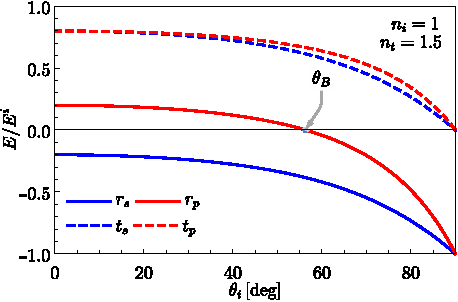
\includegraphics[scale=1]{1-Teoria/figs/1-1-ampCoefExt}
	\end{subfigure}
	\begin{subfigure}{.05\textwidth}\vspace{-4.5cm}\caption{}\label{sfig:coefInt}\end{subfigure}
	\begin{subfigure}{.43\textwidth} \hspace*{-.9cm}
	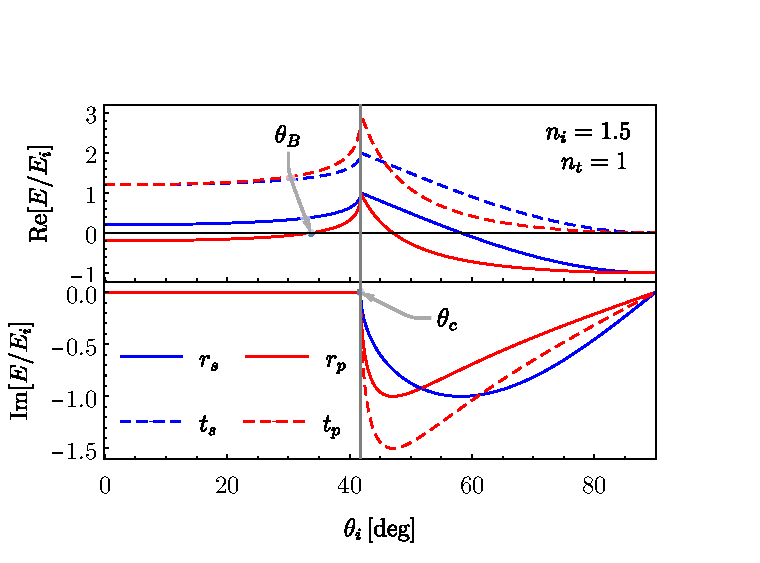
\includegraphics[scale=1]{1-Teoria/figs/1-1-ampCoefInt}
	\end{subfigure}\vspace*{-.7em}
	\caption{ Coeficientes de amplitud $r$ (líneas continuas) y $t$ (líneas discontinuas), en función del ángulo de incidencia $\theta_i$, en configuración de incidencia \textbf{a)} externa e \textbf{b)} interna para una interfaz entre  aire ($n=1$) y un medio con índice de refracción $n = 1.5$. Los cálculos para polarización  \emph{s} se muestran  en azul y  para \emph{p} en rojo; en el caso de incidencia interna, los coeficientes de amplitud son cantidades complejas y se grafica tanto su parte real, como la imaginaria. Se indica la posición tanto para el ángulo de Brewster $\theta_B$ como para el ángulo crítico $\theta_c$ mediante las flechas grises.}	\label{fig:coefAmp}	
	\end{figure}	

Para corroborar que toda la luz es reflejada en incidencia interna para $\theta_i>\theta_c$ se considera la conservación de la energía transportada por los campos EMs al cruzar la interfaz. Al calcular el promedio temporal\footnote{El promedio temporal del vector de Poynting es $\langle\vb{S}\rangle_t = (1/\tau)\int_t^{t+\tau}\vb{S}(t')dt'$, y para campos EMs tipo ondas planas es $\langle\vb{S}\rangle_t = (1/2) \Re[\vb{E}\times\qty(\vb{B}/\mu)^*]$ \cite{jackson1999electrodynamics}.\index{Poynting!vector de!promedio temporal del}} del vector de Poynting [Ec. (\ref{eq:Poynting})], se obtiene la irradiancia $I$ \cite{hecht1998optics}, dada por
	\begin{align}
	I = \langle S \rangle_t = \frac{nc\varepsilon_0}{2} EE^*,
	\label{eq:Irr}
	\end{align}
que corresponde a la energía promedio por unidad de tiempo y unidad de área  transportada por los campos EMs en la dirección $\vu{k}$ \cite{griffiths2013electrodynamics}. Para calcular la potencia $P$, definida como energía por unidad de tiempo, transportada por los campos EMs al cruzar la interfaz se multiplica la Ec. \eqref{eq:Irr} por la sección transversal de un haz de luz. En la Fig. \ref{fig:hazcircular} se muestran las secciones transversales de un haz  que incide a un ángulo $\theta_i$ sobre la interfaz entre dos medios con índice de refracción $n_i$ y $n_t$, respectivamente. Cuando el haz se refleja, a un ángulo $\theta_r=\theta_i$, y se refracta a un ángulo $\theta_t$, la sección transversal del haz cambia. Si el área de los haces justo en la interfaz es $A$, mediante la ley de reflexión [Ec. \eqref{eq:LeyReflexion}] y la ley de Snell [Ec. \eqref{eq:LeySnell}], la sección transversal del haz incidente y el reflejado  es $A\cos\theta_i$, mientras que la del haz transmitido es $A\cos\theta_t$. Al emplear la Ec. \eqref{eq:Irr} y multiplicarla por el área de cada uno de los tres haces mostrados en la Fig. \ref{fig:hazcircular}, se obtiene que la energía por unidad de tiempo transportada por cada haz de luz es
	\begin{align*}
	P = I A \cos\theta = \frac{n c \varepsilon_0}{2}  EE^* \cos\theta,
	\end{align*}
en donde el ángulo $\theta$ e índice de refracción $n$ toman los valores de $\theta_i$ y $n_i$ para el haz incidente y el reflejado, mientras que  toma los valores de $\theta_t$ y  $n_t$ para el haz transmitido. Cuando se normaliza la energía por unidad de tiempo transportada por el haz reflejado y por el haz transmitido entre la del haz incidente, se obtienen las expresiones de la reflectancia $R$ y la transmitancia $T$ \cite{hecht1998optics} \vspace{-.5em} \index{Fresnel!Reflectancia ($R$)}\index{Fresnel!Transmitancia ($T$)}
	\begin{tcolorbox}[title = Reflectancia y transmitancia]
	\eqhalf{ R =  r r^*, \label{eq:R}}
	\eqhalf{ T = \frac{n_t\cos\theta_i}{n_i \cos\theta_t} t t^*,\label{eq:T}}
	\end{tcolorbox}\vspace*{-.75em}\noindent	
en donde $r$ es el coeficiente de amplitud de reflexión y $t$ el de transmisión, dados por las Ecs. \eqref{eq:rs}--\eqref{eq:tp}.

	\begin{figure}[t]\centering
\begin{tikzpicture}[scale=.7]
%\draw (3.46,1.9) circle(2pt);ESTA ES LAREFERENCIA PARA ANTES DE MOVER LAS COSAS

%---------------------------------------------------------------------------------------- SUPERFICIE
\fill[blue!20]			
(-5,-1) -- (-3,2) 
-- (3,2) -- (5,-1)
--(-5,-1);						

\draw[dashed,gray](0,-4)--(0,5);  %---------------------------------------------------- Vertical dashed line

\node at (-4,-.5) {Medio 1 $\; n_i$}; %-------------------------------------------------- media names
\node at (-4,-1.5) {Medio 2 $\; n_t$};

%---------------------------------------------------------------------------------------- SPOT INTERFAZ
\fill[lgreen, opacity= .75] (0,.5) circle (2 and .6); 
\draw[black](0,.5) circle (2 and .6)		% -------------------------------------------  Etiqueta área
			(0,.5)node[]{$A$};	
%------------------------------------------------------------- INCIDENTE
\path[shift = {(0,1.7)}] (0,0)++(112.5:1cm)node{$\theta_i$};   %---------- Angle
\draw[latex - latex,shift = {(0,2.1)}](-1,.5)arc(144.5:90:1.1cm);

\draw [-,shift = {(-2,.5)}, rotate = 55.5] (0,0) -- (0,3.2);%Cara del cilindro(Rota desde 90°)
\draw[-, shift = {(2,.5)},rotate = 55.5] (0,0) -- (0,6.3);

\draw[black, rotate = 50.75, shift = {(0,5)}](0,0) circle (1.145 and .3);% Tapa del cilidndro del del área
\node at (-5.1,3.5) { $A\cos\theta_i$};
\fill[lgreen, opacity= .5, rotate = 50.75, shift = {(0,5)}](0,0) circle (1.145 and .3);

%-------------------------------------------------------------- REFLEJADO
\path[shift = {(0,1.7)}] (0,0)++(67.5:1cm)node{$\theta_r$};   %------------- Angle
\draw[latex - latex ,shift = {(0,2.1)}](1,.5)arc(35:90:1.1cm);

\draw [-,shift = {(-2,.5)}, rotate = -55.5] (0,0) -- (0,6.3);  %- Cara del cilindro
\draw[-, shift = {(2,.5)},rotate = -55.5] (0,0) -- (0,3.2);

\draw[black, rotate = -50.75, shift = {(0,5)}](0,0) circle (1.145 and .3); %Tapa del cilidndro del del área
\node at (5.1,3.5) { $A\cos\theta_r$};
\fill[lgreen , opacity= .5, rotate = -50.75, shift = {(0,5)}](0,0) circle (1.145 and .3);

%----------------------------------------------------------------- TRANSMITIDO
\path  (0,0)++(275:4.1)node{$\theta_t$};    %------------------------- Angle
\draw[latex - latex](0,-3.5)arc(270:290:1.5cm);

\draw [-,shift = {(-2,.5)}, rotate = 33.5] (0,0) -- (0,-5);   %------------------------- Cara del cilindro
\draw[-, shift = {(2,.5)},rotate = 33.5] (0,0) -- (0,-3.1);

\draw[black, rotate = 29.2, shift = {(.5,-3.6)}](0,0) circle (1.675 and .3);		%-------- Tapa del cilidndro del del área
\node at (3.5,-3.5) {$A\cos\theta_t$};
\fill[lgreen, opacity= .5,  rotate = 29.2, shift = {(.5,-3.6)}](0,0) circle (1.675 and .3);

\end{tikzpicture}
	\caption{Sección transversal de un haz de luz incidiendo en una interfaz entre dos medio lineales, homogéneos e isótropos con índices de refracción $n_i$ y $n_t$. El haz incide sobre la interfaz a un ángulo de $\theta_i$, se refleja con un ángulo $\theta_r$ y se transmite a un ángulo $\theta_t$, calculados mediante las leyes de reflexión y de Snell, respectivamente. El área del haz sobre la interfaz es $A$, mientras que en los haces, al propagarse, es $A\cos\theta$, en donde $\theta$ es el ángulo de propagación respectivo para cada haz.} \label{fig:hazcircular}
	\end{figure}

En la Fig. \ref{fig:frsnel} se grafican la reflectancia (líneas continuas) y transmitancia (líneas discontinuas) en función del ángulo de incidencia $\theta_i$, para polarización \emph{s} (en azul) y \emph{p} (en rojo), de un haz de luz que incide en la interfaz entre aire ($n=1$) y un medio con índice de refracción $n=1.5$, para una configuración de incidencia externa [Fig. \ref{sfig:frsnelExt}] e incidencia interna [Fig. \ref{sfig:frsenlInt}]. En la Fig. \ref{fig:frsnel} se observa que $R_p=0$ para el ángulo de Brewster, tanto para incidencia interna como externa. Asimismo, se aprecia que la relación $R+T=1$ se cumple para todo ángulo de incidencia y en particular para $\theta_i>\theta_c$ se cumple que $R_p = R_s = 1$ y que $T_s = T_p = 0$. La relación $R+T=1$ es válida ya que se consideraron medios materiales sin absorción. En general, la función dieléctrica ($\varepsilon=n^2$, para medios no magnéticos) es compleja, donde la parte imaginaria   $\Im[\varepsilon]$ se asocia con la absorción de energía por el material \cite{ibach2003solid}. Cuando la luz se propaga a través de algún medio absorbente, se cumple en general 
	\begin{align*}
	R + T + A = 1,
	\end{align*}
en donde el término $A$ es la energía absorbida por el material, relativa a la energía del haz incidente.\index{Función dieléctrica!Absorción}
%
\begin{figure}[t!]\centering\hspace*{-1.5em}
	\begin{subfigure}{.05\textwidth}\vspace{-4.5cm}\caption{}\label{sfig:frsnelExt}\end{subfigure}
	\begin{subfigure}{.43\textwidth} \hspace*{-.7cm}
	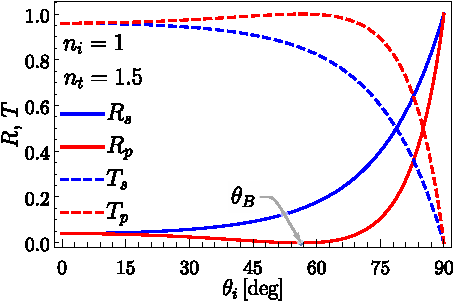
\includegraphics[scale=1]{1-Teoria/figs/1-2-FrsnelExt}
	\end{subfigure}
	\begin{subfigure}{.05\textwidth}\vspace{-4.5cm}\caption{}\label{sfig:frsenlInt}\end{subfigure}
	\begin{subfigure}{.43\textwidth} \hspace*{-.7cm}
	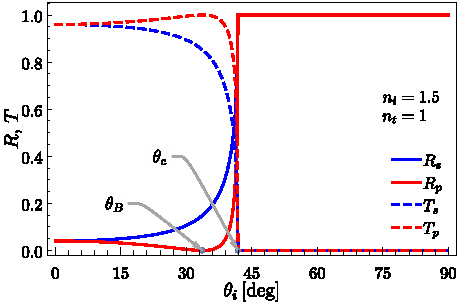
\includegraphics[scale=1]{1-Teoria/figs/1-2-FrsnelInt}
	\end{subfigure}\vspace*{-.7em}
	\caption{  Reflectancia (líneas continuas) y transmitancia (líneas discontinuas) en función del ángulo de incidencia $\theta_i$, en configuración de incidencia \textbf{a)} externa y \textbf{b)} interna para una interfaz entre  aire ($n=1$) y un medio con índice de refracción $n = 1.5$. Los cálculos para polarización  \emph{s} se muestran  en azul y  para \emph{p} en rojo. Se indica la posición tanto del ángulo de Brewster $\theta_B$, como del ángulo crítico $\theta_c$ mediante las flechas grises.}	\label{fig:frsnel}	
	\end{figure}	
%